\documentclass{article}
\usepackage{graphicx} % Required for inserting images
\usepackage{amsmath}
\usepackage{breqn}
\usepackage{xcolor}
\usepackage{tikz}
\usepackage{tcolorbox}
\usepackage{comment}
\usepackage{subcaption}
\usepackage[utf8]{inputenc}
\usepackage{float}
\usepackage{placeins}

\title{Oscillations forcées}
\author{Hervé SV}
\date{June 2023}

\begin{document}

\maketitle

Les constantes sont supposées positives sauf si contre-indiqué

\section{Oscillations amorties}

L'équation différentielle pour un oscillateur harmonique avec variable $x$ :
\[ \ddot{x} + \omega_0^2 x = 0 \]

Dans le cas d'un oscillateur harmonique en présences d'une force résistive (qui dépend de la vitesse) :

\[ m\ddot{x} = -m\omega_0^2 x - m\gamma \dot{x} \]

On trouve donc :

\[ \ddot{x} + \gamma \dot{x} + \omega_0^2 x= 0 \]

On cherche la solution homogène (la solution particulière est nulle).
L'équation caractéristique :

\[ r^2 + \gamma r + \omega_0^2 = 0 \]
\[ \Delta = \gamma^2 - 4\omega_0^2 \]

On s'intéresse au cas $\omega_0 > \gamma/2$

\begin{dmath*}
    r  = \frac{-\gamma \pm \sqrt{\gamma^2 - 4\omega_0^2}}{2}\\
    = -\gamma/2 \pm i\sqrt{\omega_0^2 - \gamma^2/4}
\end{dmath*}

le système va donc osciller à une fréquence différente de $\omega_0$ : 

\[ \omega = \sqrt{\omega_0^2 - \gamma^2/4} \]

\begin{tcolorbox}
\[ x = e^{-\frac{\gamma}{2}t}(A\cos(\omega t) + B\sin(\omega t)) \]
\end{tcolorbox}

On a une oscillation sinusoïdale avec une amplitude qui décroît de manière exponentielle. On voit que $x$ tend vers 0 pour grand $t$.

\section{Oscillations forcées}

Étudions le cas où l'on 
applique une force supplémentaire $F$. Si $F$ est de la forme $F_0\cos(\omega t)$
\[ \ddot{x} + \gamma \dot{x}+ \omega_0^2 x = \frac{F_0}{m}\cos(\omega t)=f_0\cos(\omega t) \]

On passe par les complexes pour trouver la solution particulière :

\[ x = Ae^{i\omega t}, \quad \cos(\omega t) = \Re(e^{i \omega t}) \]



\[ (-\omega^2 + i \omega\gamma + \omega_0^2)x = f_0 e^{i \omega t} \]



\begin{dmath*}
x = \frac{1}{\omega_0^2 -\omega^2 + i \omega\gamma} f_0 e^{i\omega t} \\
= Rf_0 e^{i \omega t}
\end{dmath*}

\[ R = \frac{1}{\omega_0^2 -\omega^2 + i \omega\gamma} = \rho e^{i\phi} \]

C'est-à-dire que $x$ est égale à la force (divisé par un facteur de masse) multiplié par une valeur complexe $R$.
Le module $\rho$ est un multiplicateur de l'ampltitude de la réaction suite à la force, et l'argument $\phi$ va induire un déphasage de $x$ par rapport à la force.

\[ x  = \rho f_0 e^{i(\omega t + \phi)} \]

En revenant dans les réelles

\[ x  = \rho f_0 \cos(\omega t \phi)\]


Sachant qu'un complexe quelconque multiplié par son conjugé donne le carré du module :

\begin{dmath*}
    RR^* = \rho^2 \\
    = \frac{1}{(\omega_0^2 -\omega^2 + i \omega\gamma)(\omega_0^2 -\omega^2 - i \omega\gamma)}
    = \frac{1}{(\omega_0^2 - \omega^2)^2 + \omega^2\gamma^2}
\end{dmath*}

Pour trouver $\phi$, on peut prendre la réciproque de $R$ pour trouver une expression plus sympa pour la partie réelle et imagninaire.
\begin{dmath*}
    \frac{1}{R} = \frac{1}{\rho}e^{-i\phi} \\
    = \omega_0^2 -\omega^2 + i\omega\gamma
\end{dmath*}

\[ \tan(-\phi) = \frac{\Im(1/R)}{\Re(1/R)} \]
\[ \tan(\phi) = \frac{-\omega\gamma}{\omega_0^2 - \omega^2} \]


\begin{comment}
\[ \phi = 
\begin{cases}
    \arctan(\frac{-\omega\gamma}{\omega_0^2 - \omega^2}) & \text{si } \omega < \omega_0 \\
    \arctan(\frac{-\omega\gamma}{\omega_0^2 - \omega^2}) - \pi & \text{si } \omega > \omega_0
    
\end{cases}
\]

L'image d'$arctan$ n'est que défini sur $]-\frac{\pi}{2}, \frac{\pi}{2}[$, d'ou le terme correcteur $-\pi$
\end{comment}


\begin{figure*}[h]
    \centering
    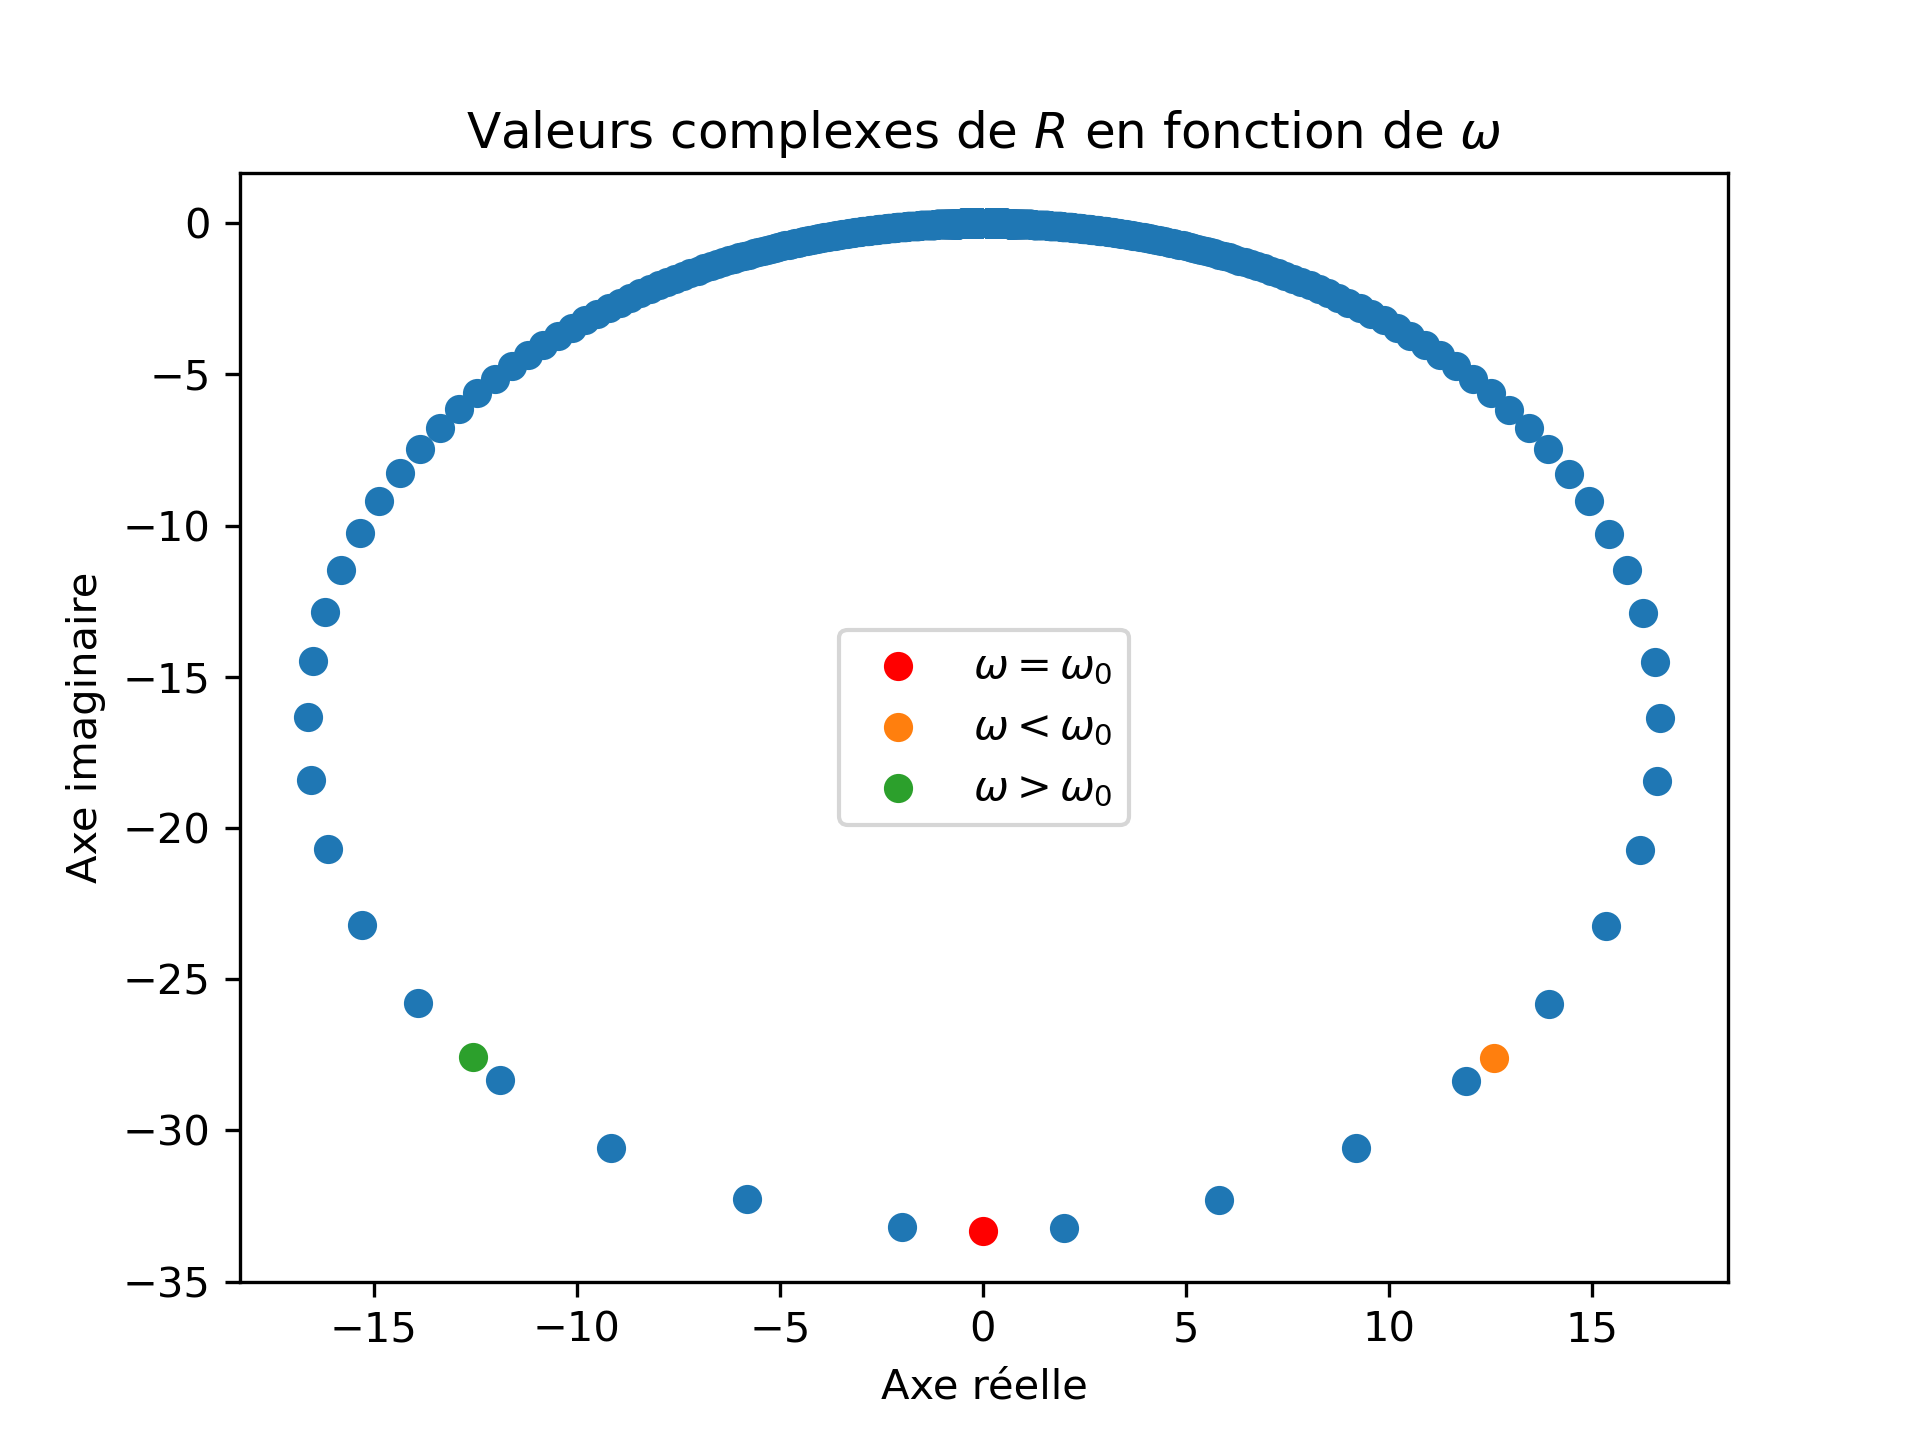
\includegraphics[scale=0.6]{figs/R_valeurs.png}
    \caption{$\rho$ atteint son maximum lorsque $\omega = \omega_0$. Le déphasage $\phi$ prend des valeurs entre $0$ et $-
    \pi$ radians}
\end{figure*}

\begin{figure*}[h]
    \centering
    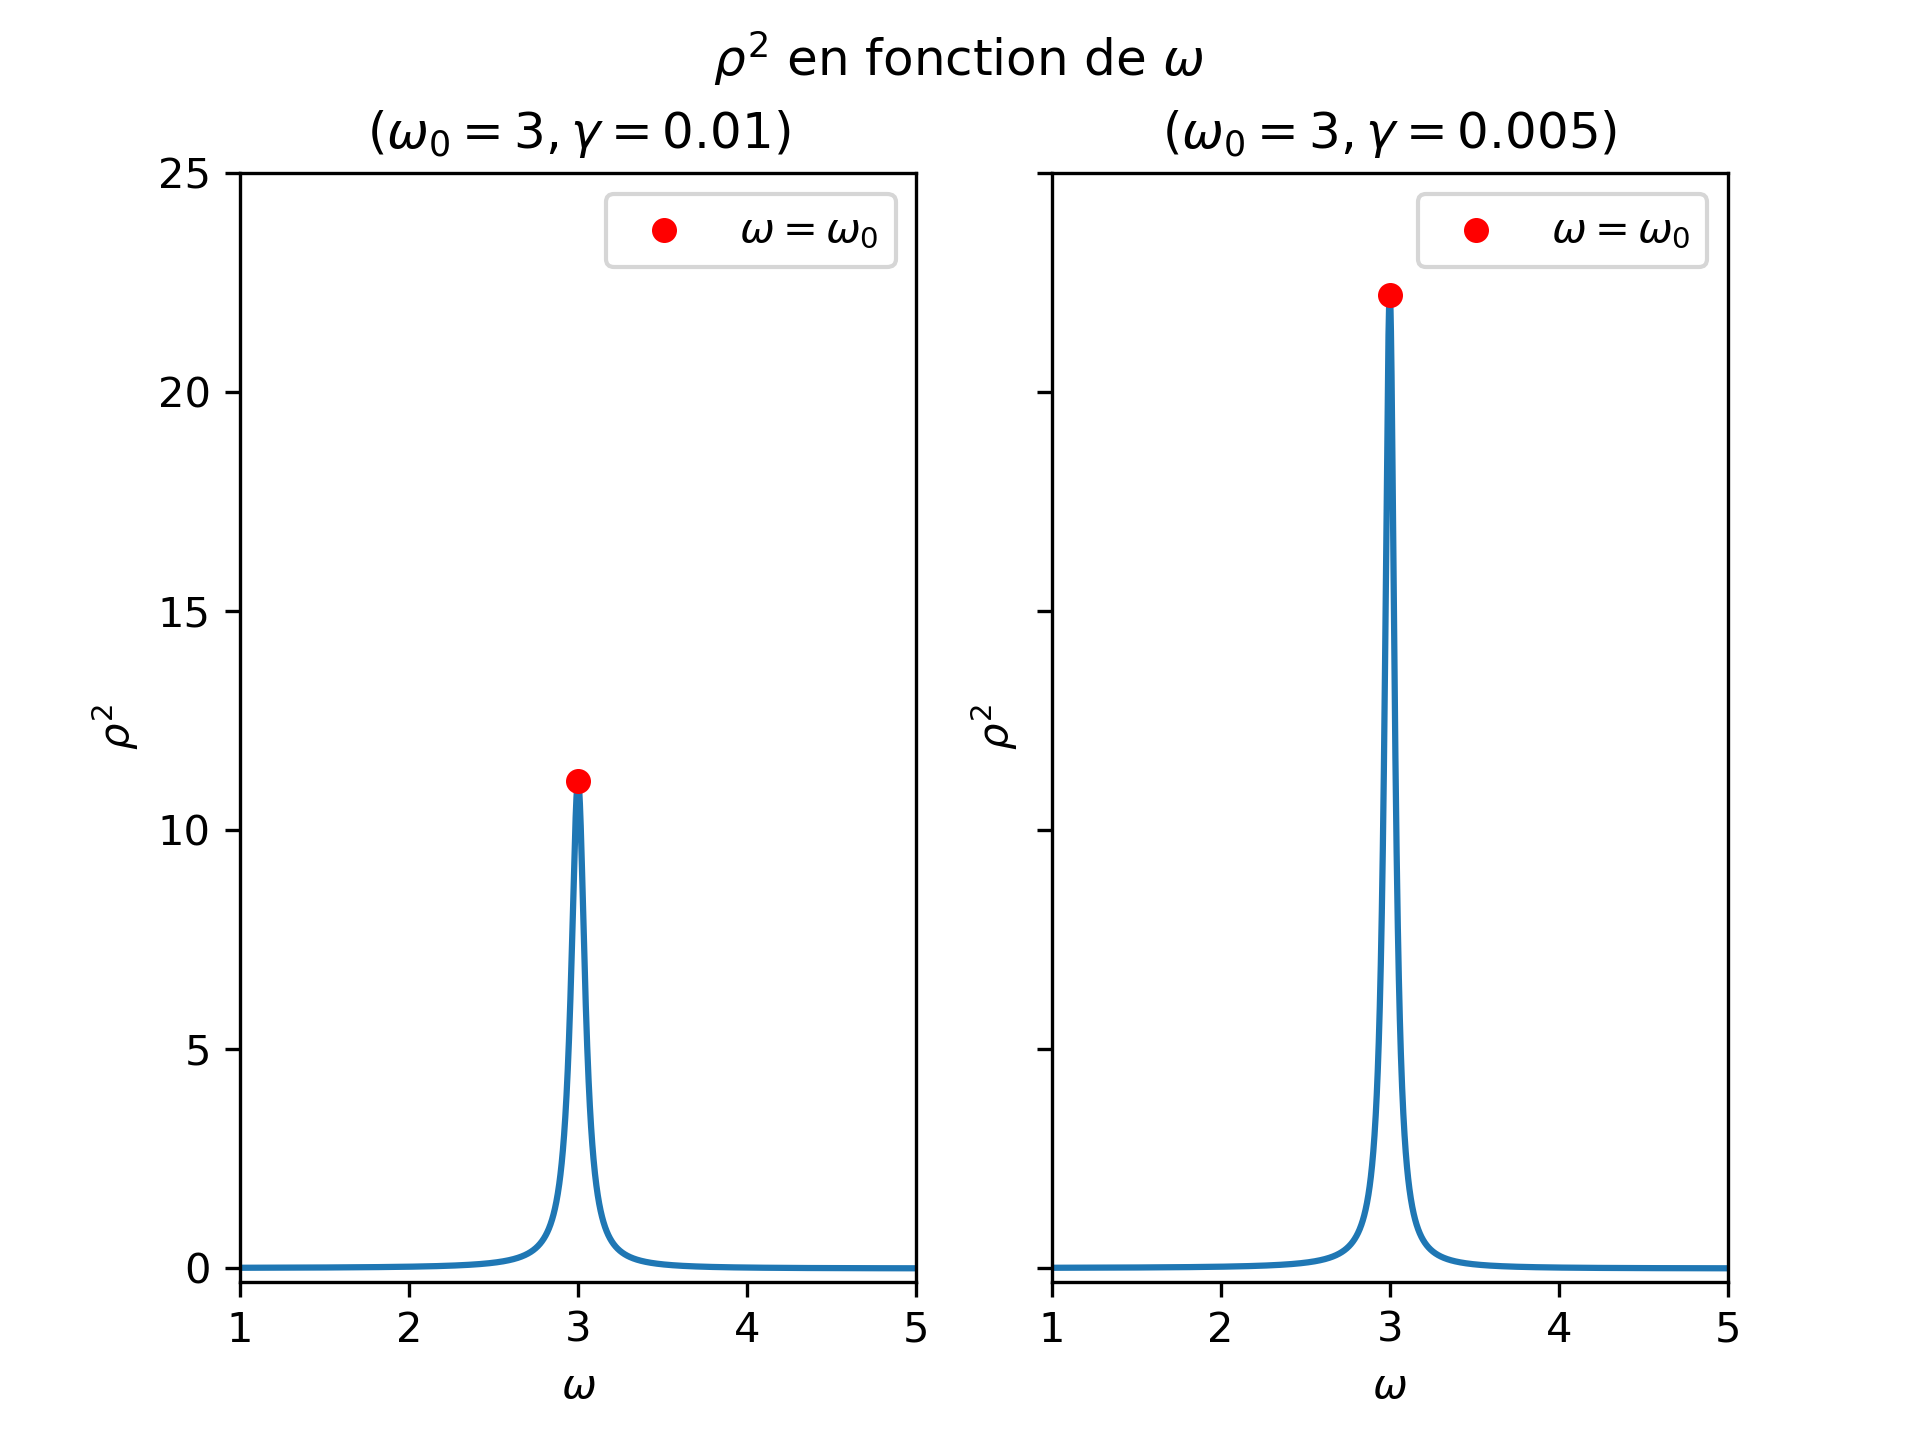
\includegraphics[scale=0.7]{figs/rho_plot_contrast.png}
    \caption{Plus $\gamma$ est faible plus la courbe est pentue, et plus l'oscillateur va être selective avec la valeur de la pulsation $\omega$}
    \centering
\end{figure*}

\FloatBarrier

$\rho^2$ prend la forme d'une courbe lorentzienne, l'amplification de la force est très forte lorsque $\omega$ est proche de $\omega_0$, de même l'amplification tend vers zero le plus $\omega$ s'éloigne de $\omega_0$

On dit que c'est un système résonant car elle privilegie une faible gamme de et ne répond quasiment pas au fréquences en dehors de cette gamme centré autour de $\omega_0$.

En additionant la solution homogène et la solution particulière, on trouve notre solution génerale de la forme.
\[ x = Ae^{i\omega t}, \quad \cos(\omega t) = \Re(e^{i \omega t}) + \rho f_0 \cos(\omega t \phi) \]
Puisque la solution homogène tend assez rapidement vers zéro, après ce court état transient, on retrouve 


On peut aussi définir un facteur de quality
\[ Q = \frac{\omega_0}{\Delta\omega} \]

Lorsque $\omega \approx \omega_0$, 



\section{Étude de cas : circuit RLC}

\end{document}

